
\chapter{Results}

The following results are exploratory in nature, and After some poor initial results the focus was laid on proving that
the network can perform at all, rather than fine-tuning hyperparameters towards optimal performance. This decision was
in part motivated by a priorization of gaining neuroscientific insights over proving high performance. Yet it should be
noted, that training the network is computationally quite costly (c.f. Section \ref{sec-benchmark}), which turned
parameter studies into a time-consuming process. The network is furthermore fairly sensitive to changes in
parametrization, hence many early experiments in this direction immediately caused a failure to learn. The search for
default parameters itself took some effort, as a certain heterogeneity exists in the two existing implementations
\citep{sacramento2018dendritic,Haider2021}, both in hyperparameters as in the simulation environment. This model
includes properties of both variants, while relying more strongly on the Latent Equilibrium implementation. Unless
stated otherwise, neurons employ prospective activation functions in all simulations. So far, no drawbacks to this
mechanism have presented themseleves, and learning speed can be increased drastically compared to the original
implementation. The full default parametrization is shown in Table \ref{tab-params}.

Since it was anticipated that the spiking implementation would perform worse than the rate-based variant, the first
goal was to measure how big this difference in performance is. Furthermore, a relevant question was, to what degree
the synaptic delays enforced by NEST would influence performance of the rate model. These questions will be answered
in the part of the upcoming sections.




\section{The self-predicting state}

As a first comparison between the three implmementations, the pre-training towards a self-predicting state (cf.
\cite{sacramento2018dendritic}[Fig. S1]) was performed. For this experiment, no target signal is provided at the output
layer, and the network is tasked with learning to self-predict top-down input. The network is initialized with fully
random weights and stimulated with random inputs from a uniform distribution between 0 and 1. A comparison of the
four error metrics between networks is shown in Fig. \ref{fig-self-pred}.



\begin{figure}[t]
    \centering
    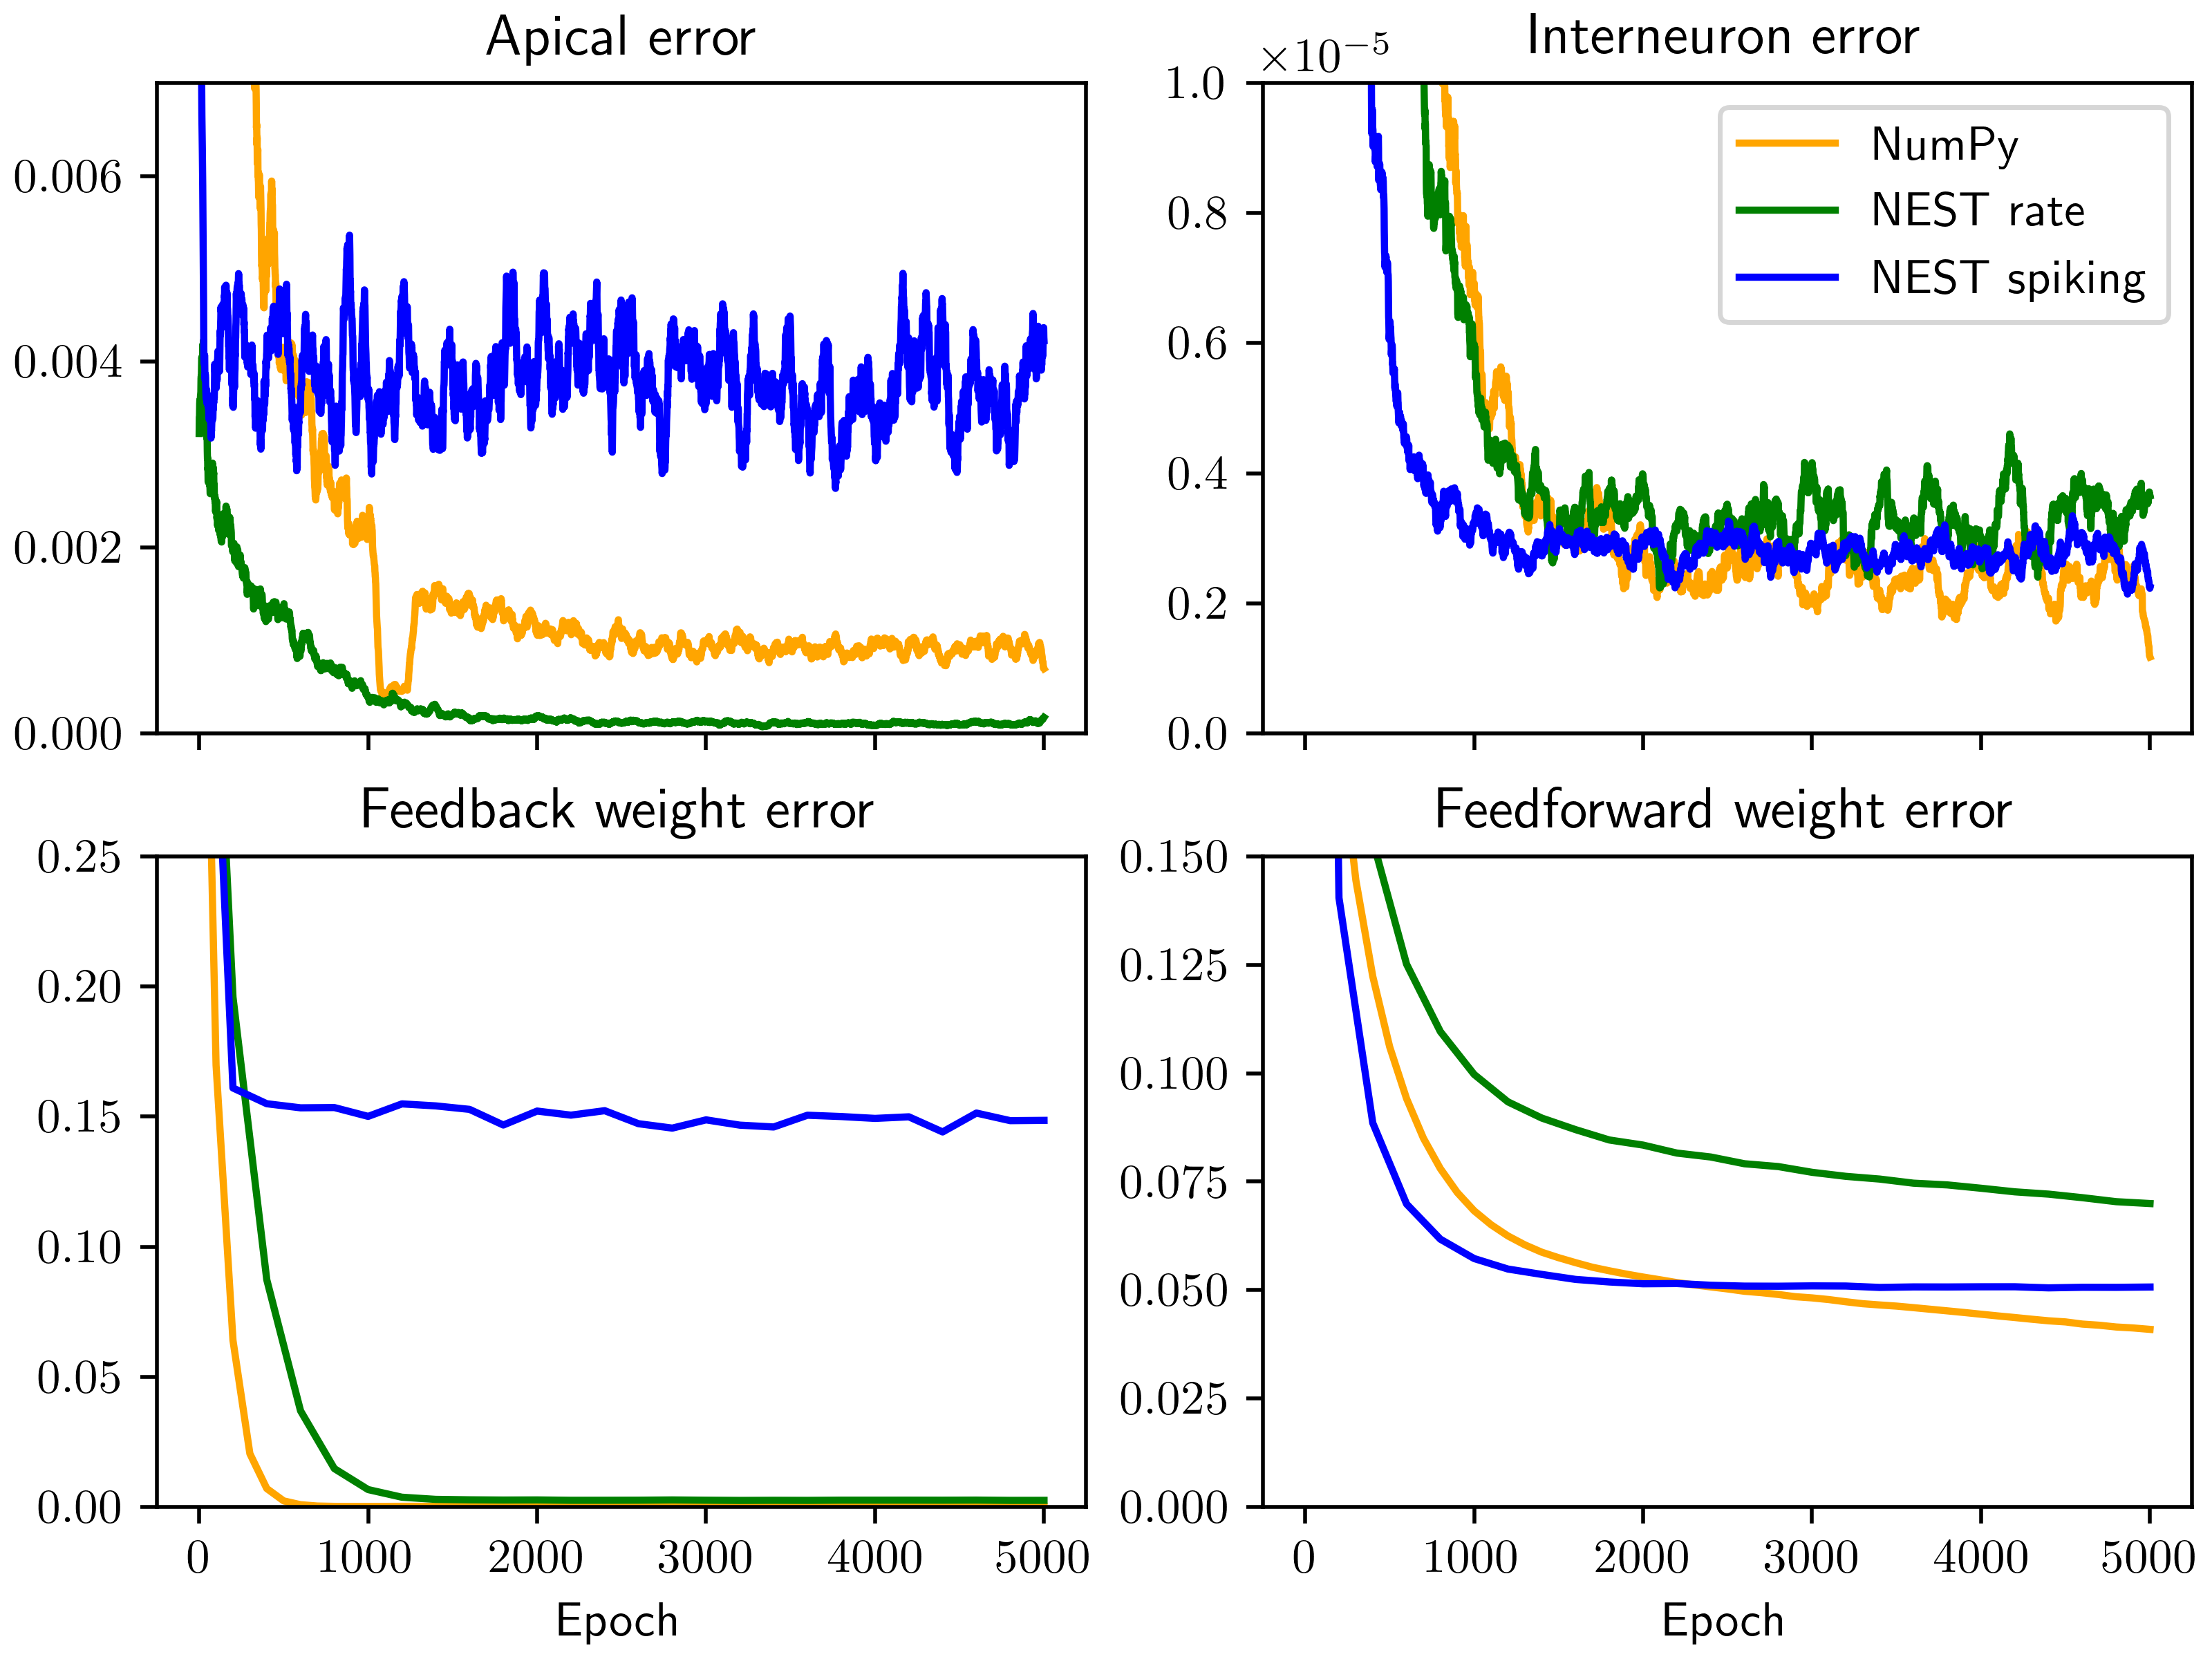
\includegraphics[width=0.9\textwidth]{fig_self_prediction}
    \caption{Different network types learn to predict self-generated activity in superficial layers. All networks were
        initialized with the same random weights for dimensions $[5, 8, 3]$, and stimulated with $5000$ samples of
        random input for $100ms$ each. As described in \cite{sacramento2018dendritic}, during this phase only
        Pyramidal-Interneuron and Interneuron-Pyramidal weights are plastic ($\eta^{pi}=0.05, \eta^{ip}=0.02375,
            \eta^{up}=\eta^{down}=0$). For spiking neurons, stability was increased by setting $\psi=150$.\todo{redo figure with less smoothing and tighter yscale}}
    \label{fig-self-pred}
\end{figure}

Both rate neuron implementations were able to reach comparable values for all error metrics after roughly the same
time. The exact values that errors converge on differs slightly between implementations, with no implementation being
clearly superior. This is an important result for upcoming experiments, as it indicates that the simulation environment
developed for the NEST version is an adequate replica of the original framework.

For the spiking variant, Interneuron- and its corresponding feedfworward weight error are comparable to the other
implementations. In fact these metrics appear to converge slightly faster to comparable values. The primary limitation
of this version are the apical error and the closely correlated feedback weight error. After appearing to converge very
quickly, the two metrics stagnate at very high levels. This behaviour can at least in part be attributed to individual
spikes causing fluctuations in apical potentials. This was confirmed by repeating the experiment with $\psi=1500$, which
alleviated the issue somewhat (results not shown). Yet, error values were still inferior to the rate models, and this
change came at the cost of substantially increased training time. Therefore, this approach was not pursued much further.
A different possible solution is, to increase the membrane capacitance of the apical compartment in order to smoothe
out the error induced by individual spikes. This will be discussed in Section \ref{sec-c-m-api}.

In most simulations in the literature, the network is initialized to an ideal self-predicting state. Furthermore
feedback weights are often non-plastic ($\eta^{pi}=\eta^{down}=0$). Therefore, a failure to reduce these errors further
might not be a substantial issue. For the time being, showing that the network approaches a self-predicting state was
deemed a sufficient result.


\section{Presentation times and latent equilibrium}\label{sec-le-tpres}

In order to validate the performance of the NEST implementations on a learning task, the parameter study from
\citep{Haider2021}[Fig. 3] was replicated. In this experiment, the network is trained different stimulus presentation
times $t_{pres} \in \{0.3,\ 500\}ms$. Performance of the original Dendritic error network is compared to the improved
model which employs Latent equilibrium. Due to the costly computation of the network under such long $t_{pres}$, a
simple artificial classification dataset was developed. The \textit{Bars-dataset} is defined for $3\times3$ input- and
$3$ output neurons. it consists of three horizontal, three vertical, and two diagonal bars in the $3\times3$ grid, which
are to be encoded in a 'one-hot-vector' at the output layer. In the experiment, networks of $9-30-3$ pyramidal neurons
per layer were trained for 1000 Epochs of 24 samples each. Networks were initialized to the self-predicting state and
only feedforward $Pyr\rightarrow Pyr$ and $Pyr \rightarrow Intn$ synapses were plastic. Learning rates scaled inversely with
presentation times: $\eta^{ip}_0 = \frac{0.2}{t_{pres}}, \eta^{up}_0 = \frac{0.5}{t_{pres}}, \eta^{up}_1 =
\frac{0.1}{t_{pres}}$. The results for the NEST network using spiking neurons with default parameters
\todo{elaborate on this} are shown in Fig. \ref{fig-bars-le-snest}, while the results for NumPy and Rate NEST variants
are depicted in Supplementary Figures \ref{fig-bars-le-numpy} and \ref{fig-bars-le-rnest}, respectively.


\begin{figure}[h]
    \centering
    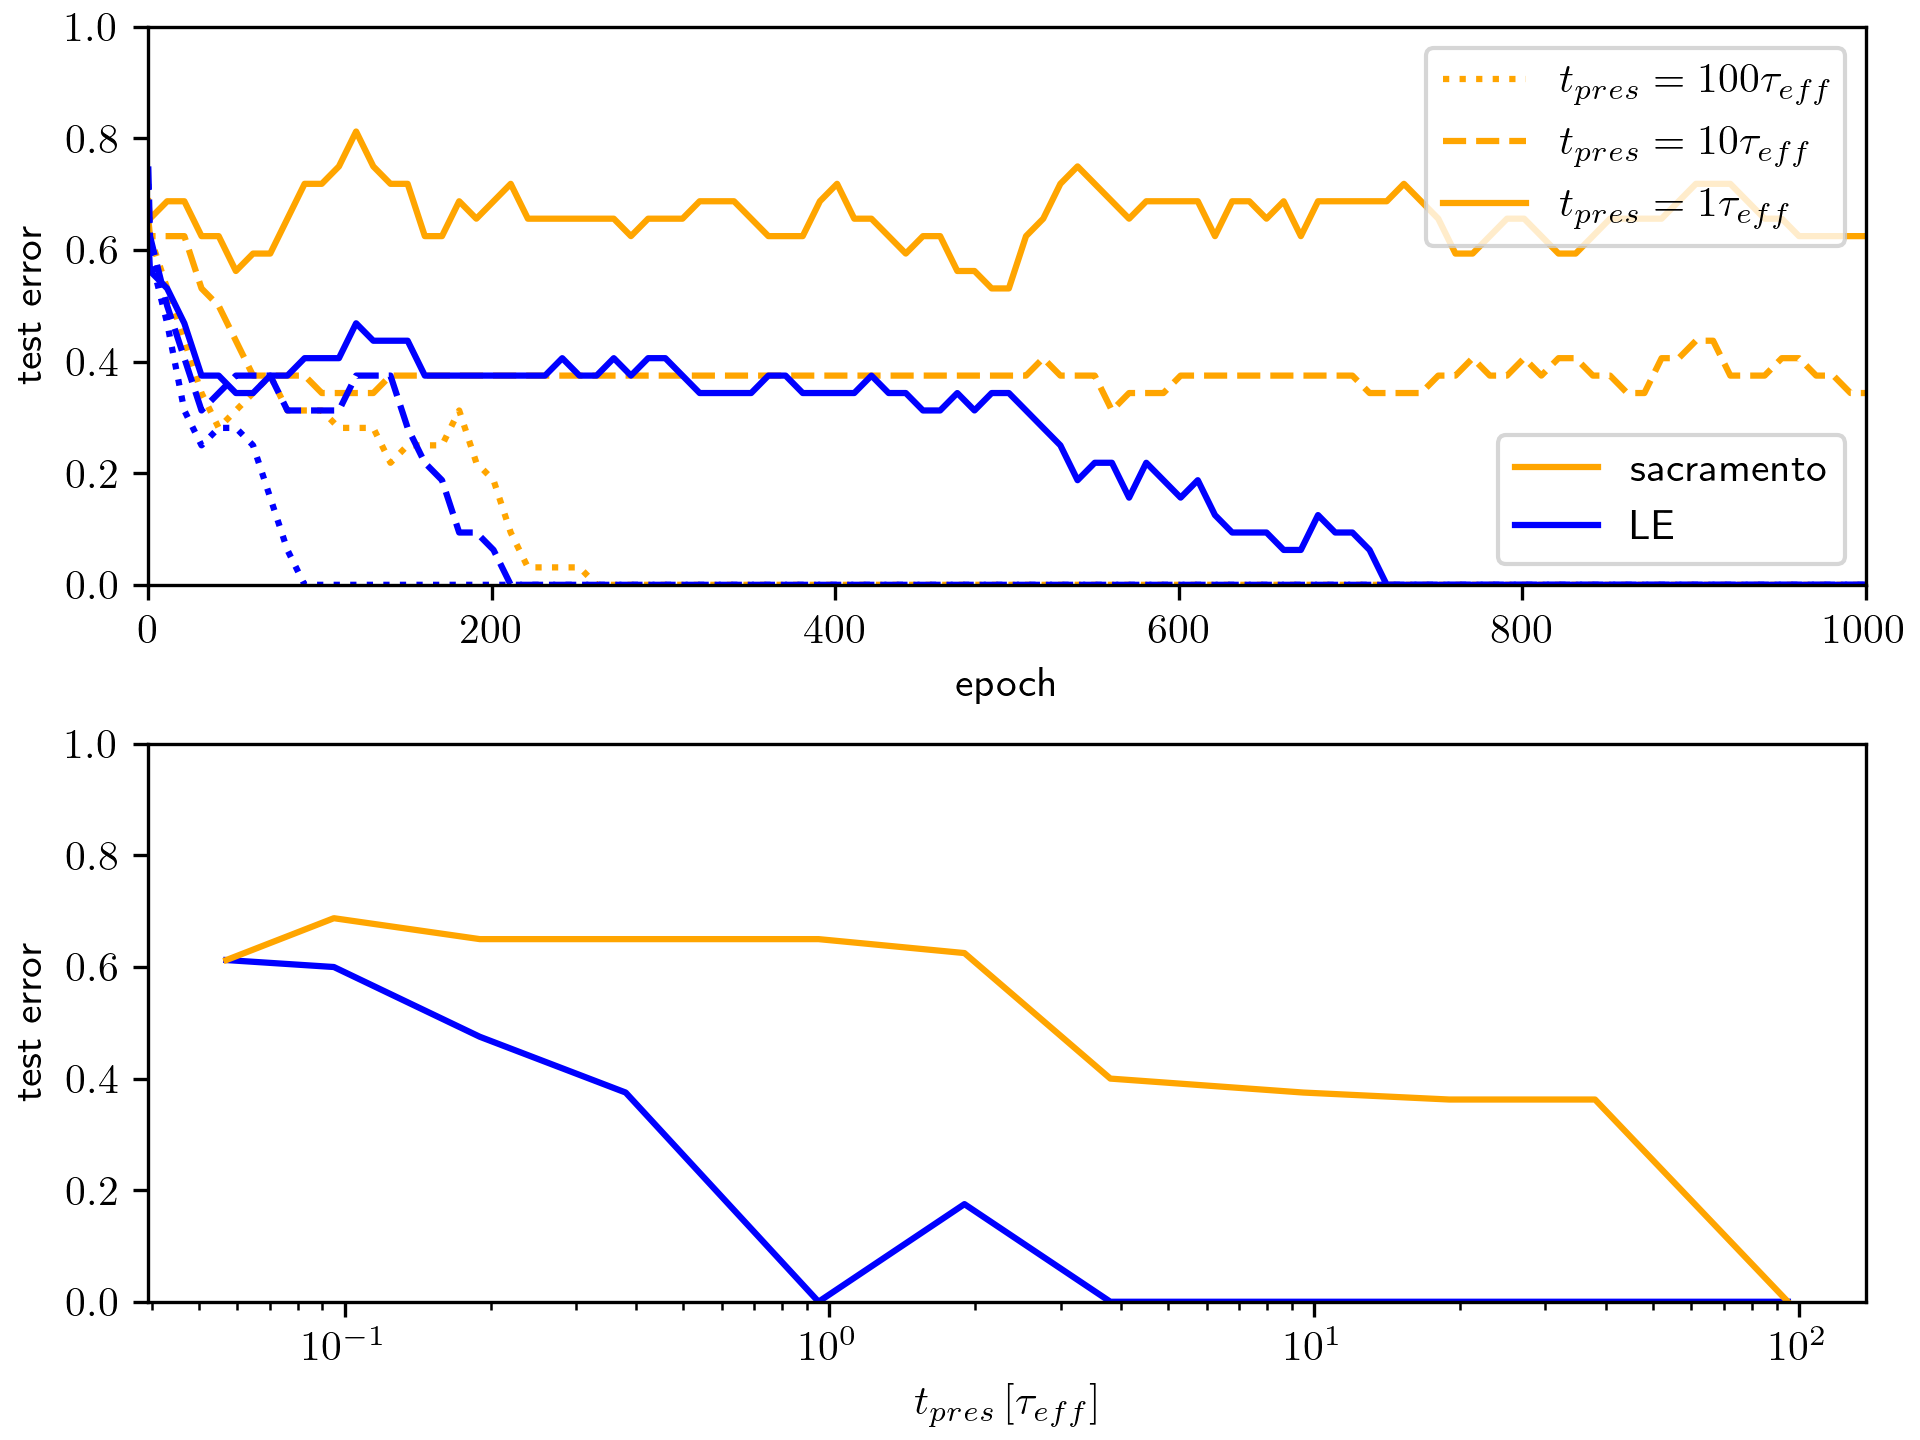
\includegraphics[width=0.9\textwidth]{fig_3_snest}
    \caption{Replication of Fig. 3 from \cite{Haider2021} using networks of spiking neurons in the NEST simulator.
        \textbf{A:} Comparison between Original pyramidal microcircuit network by \cite{sacramento2018dendritic} and
        Latent equilibrium variant from \cite{Haider2021}. Shown is the training of networks with 9-30-3 neurons on the
        Bars-dataset from with three different stimulus presentation times. \textbf{B:} Test
        performance after 1000 Epochs as a function of stimulus presentation time. }
    \label{fig-bars-le-snest}
\end{figure}

For the original dendritic error model, performance in all three implementations is close to being identical. This an
important finding as it answers two open questions: Changes made for a NEST-compatible implementation were adequate and
result in equal learning performance between rate-based implementations. Learning behaviour of the spiking model is the
same, confirming the hypothesis that the spike-based dendritic plasticity model is capable of more complex credit
assignment tasks than previously shown. In this regard, the implementation can be considered a success. 

The results for the Latent equilibrium experiments are somewhat more interesting. For very long $t_{pres}$, both rate
implementations behave the same. yet the NEST implementation requires considerably more epochs for training, as
$t_{pres}$ is reduced. In the limit, the NEST implementation was expected to break due to the enforced synaptic delay.
The NumPy variant computes a full forward pass of the network during the first simulation step, as all layers are
processed in sequence. Only feedback signals from pyramidal neurons are delayed by one timestep, in this simulation
backend. In NEST, all connections have a minimum synaptic delay of $\Delta t$. Therefore, for very short presentation
times the NEST network can not be expected to perform well. It remains an open question whether this feature alone
explains the gradual decrease in performance, or if there is an undiscovered error within the novel neuron models or
simulation environment. Such short stimulus presentation times - while exceptionally beneficial to computational
efficiency - are themselves questionable  in terms of biological plausibility, as they are much lower than pyramidal
neuron time constants \citep{McCormick1985}. Thus, no attempts were made to improve performance for very low $t_{pres}$.

The spiking variant proved similarly sensitive to presentation times as the other NEST variant. While obtaining similar
performance, it required - at best - twice as many stimulus presentations as its direct competitor. This is result, 
while somewhat expected, makes the implementation \todo{}



\section{Apical compartment capacitance}\label{sec-c-m-api}


Alternatively, increasing the membrane capacitance of the apical compartment also solves the issue as it smoothes out
the effect of individual spikes. Yet this solution also increases the relaxation period of the entire network, requiring
a highly undesirable increase in $t_{pres}$ for successful learning. Since weight errors converge to similar values as
the rate-based implementations, an increased absolute apical compartment voltage was deemed tolerable.




\section{Separation of synaptic polarity}
\todo{investigate dales law \citep{Barranca2022}}

A key limitation of the present network model is the requirement that all synapses must be able to assume both positive
and negative polarities. When restricting any synaptic population in the network to just one polarity, the network is
unable to reach the self-predicting state \todo{expand?}. Thus, activity in any neuron must be able to have both
excitatory and inhibitory postsynaptic effects facilitated by appropriate synaptic weights. This requirement is at odds
with biology, which dictates a singular synaptic polarity for all outgoing connections of a neuron, determined by neuron
type and its corresponding neurotransmitter \citeme.


To investigate to what degree the plasticity rule can deal with this constraint, an experiment was conducted: A
population of pyramidal neurons $A$  was connected to another population $C$ with plastic synapses that were
constrained to positive weights. In order to facilitate the required depression, $A$ was also connected to a population
of inhibitory interneurons $B$ through excitatory synapses with random and non-plastic weights. The interneurons in
turn were connected to $C$ through plastic, inhibitory connections. All incoming synapses at $C$ targeted the same
dendritic compartment. When inducing a dendritic error in that compartment, all plastic synapses in the network
collaborated in order to minimize that error. When injecting a positive basal error for example, the inhibitory weights
($C \rightarrow B$) decayed, while excitatory synaptic weights ($A \rightarrow B$) increased. Flipping the sign of that
error injection had the opposite effect on weights, and likewise cancelled the artificial error. This shows that a
separation of synaptic polarity does not interfere with the principles of the Urbanczik-Senn plasticity when depression
is facilitated by interneurons.

\begin{figure}[t]
    \centering
    \begin{minipage}{0.2\textwidth}
        \textbf{a)}\par\medskip
        \centering
        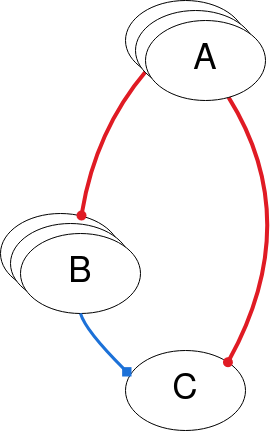
\includegraphics[width=0.9\textwidth]{fig_exc_inh_network}
    \end{minipage}\hfill
    \begin{minipage}{0.7\textwidth}
        \textbf{b)}\par\medskip
        \centering
        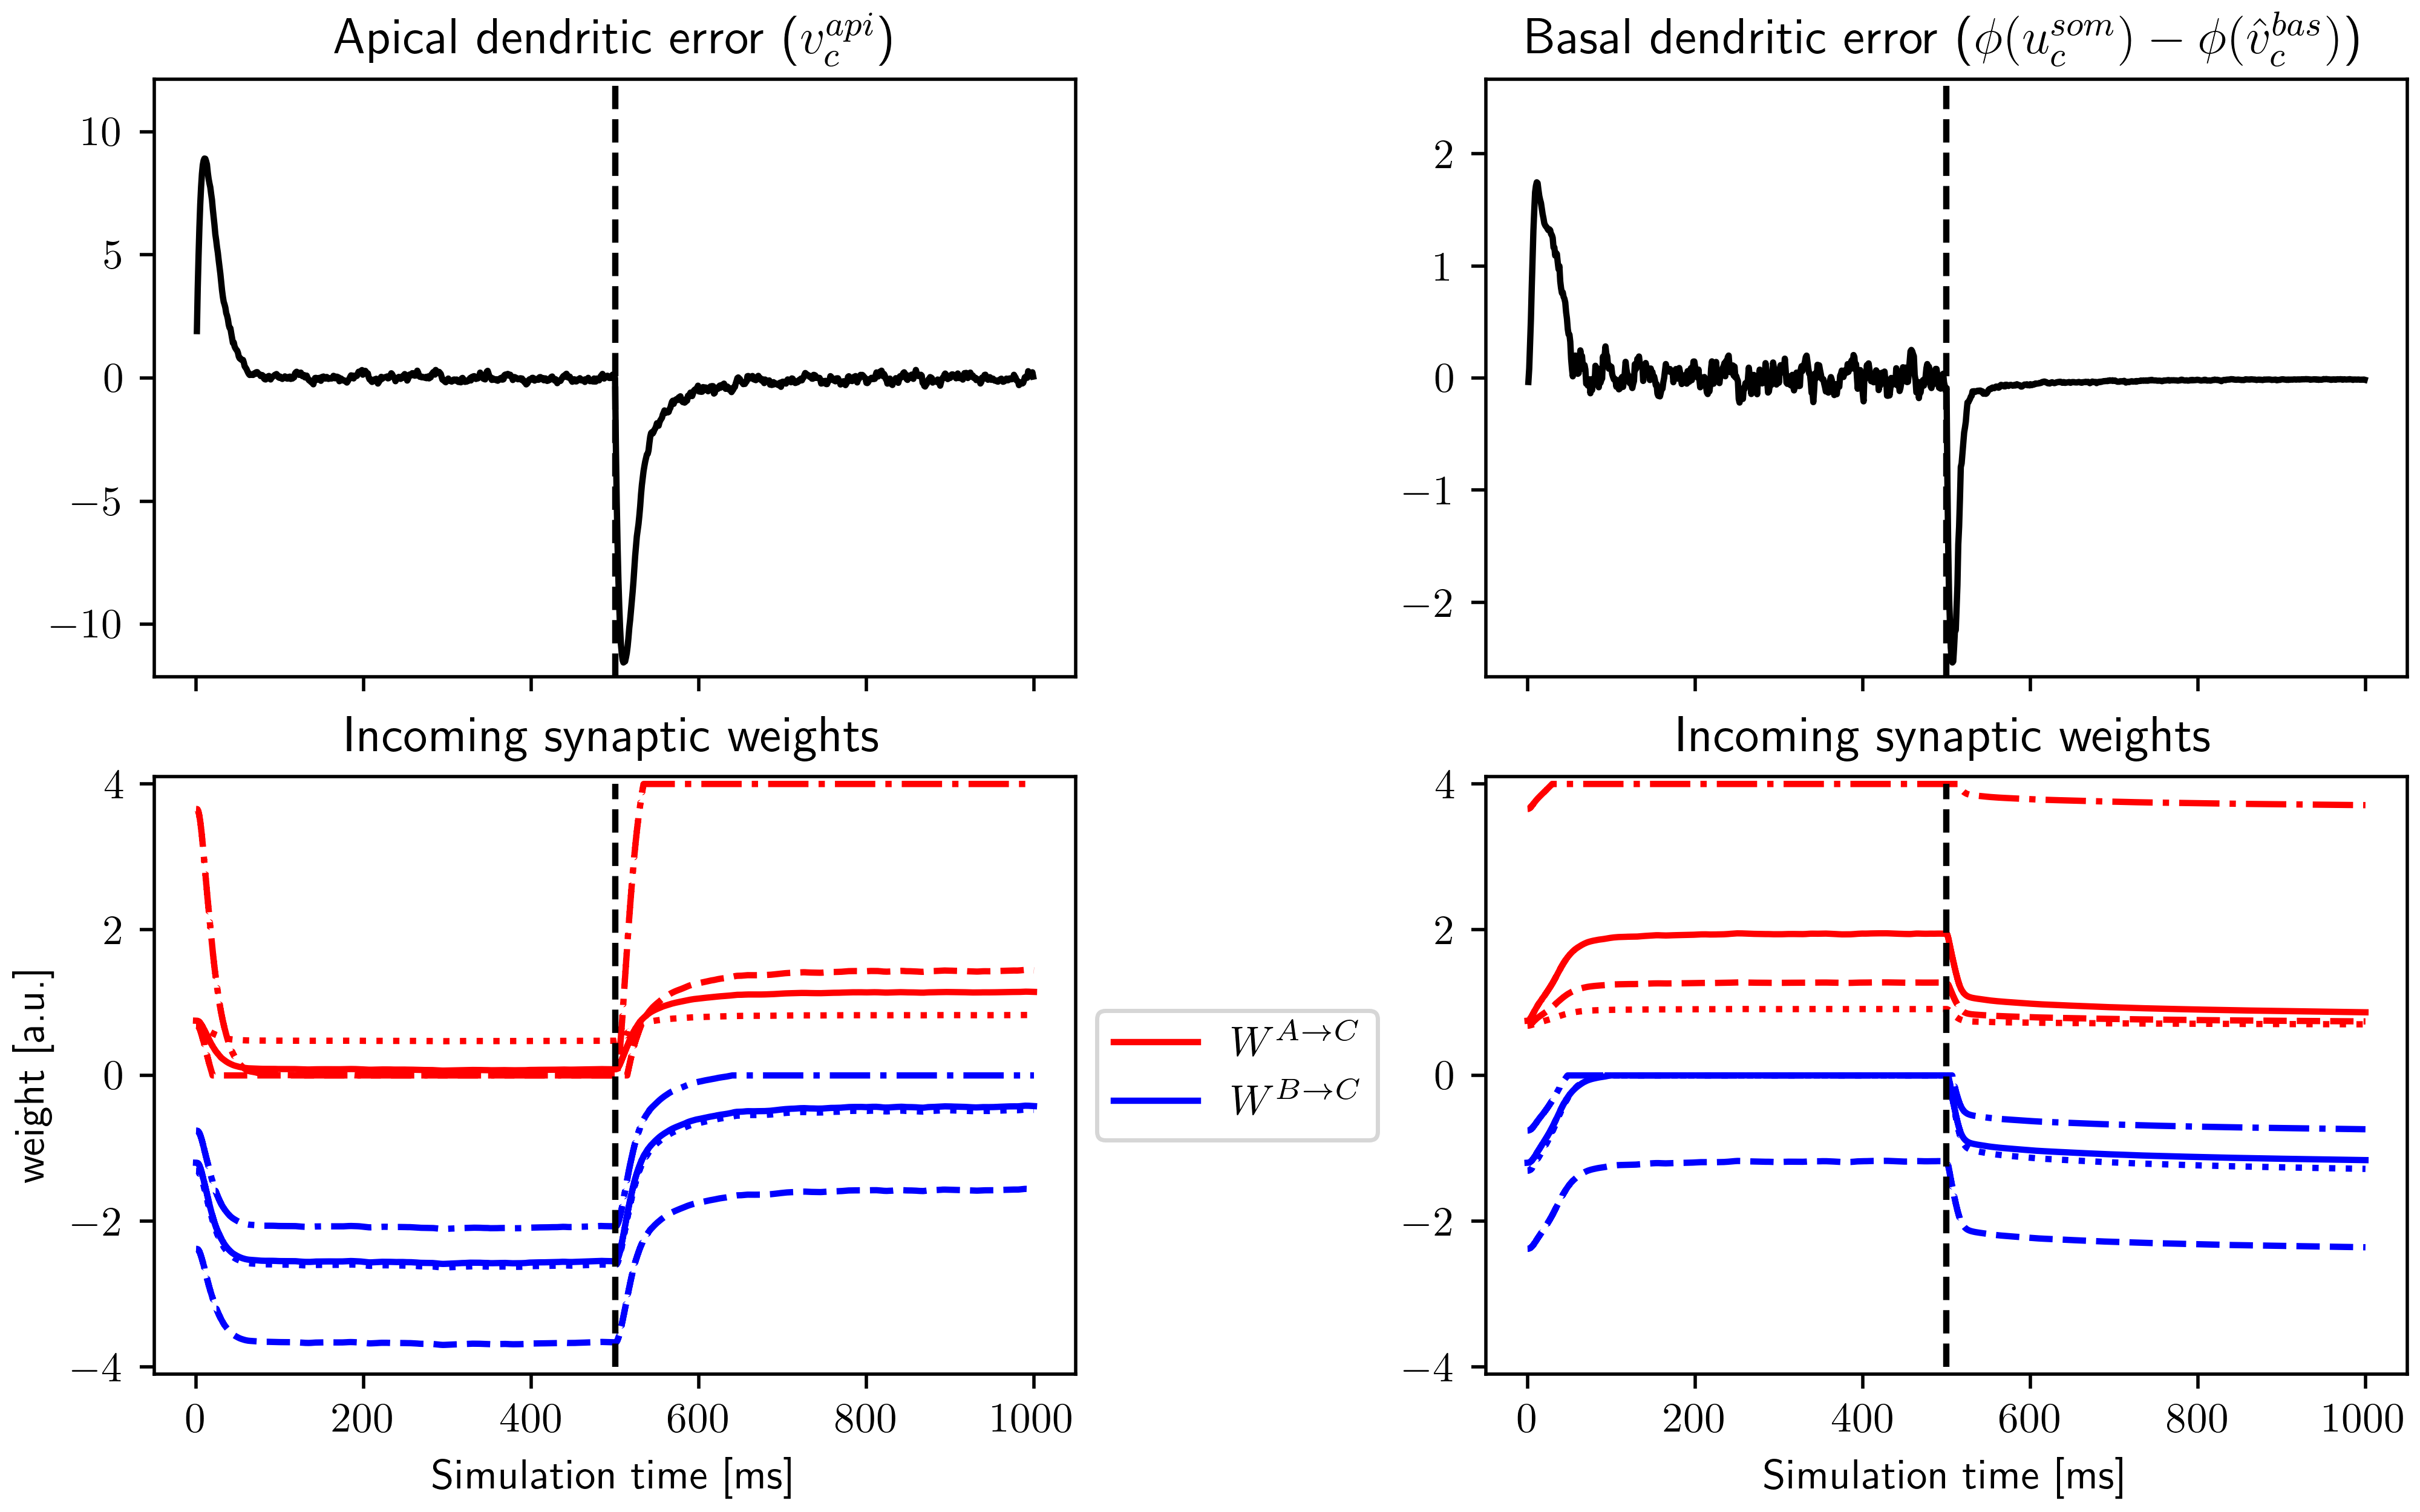
\includegraphics[width=0.9\textwidth]{fig_exc_inh_split}
    \end{minipage}
    \caption{Dendritic error minimization under biological constraints on synaptic polarity and network connectivity.
        \textbf{a)} Network architecture. An excitatory population $A$ connects to a dendrite of Neuron $C$ both
        directly and through inhibitory interneuron population $B$. Only synapses $A\rightarrow C$ and $B \rightarrow C$
        are plastic through dendritic error rules. Populations $A$ and $B$ are fully connected with random weights.
        \textbf{b)} \textit{Left:} All plastic synapses arrive at apical dendrites and evolve according to Equation
        \ref{eq-delta_w_pi}. \textit{Right:} Identical network setup, plasticity for synapses at basal dendrites
        (Equations \ref{eq-delta_w_up}, \ref{eq-delta_w_ip}). \textit{Top:} Dendritic error of a single target neuron.
        Errors of opposite signs are induced at $0$ and $500ms$ (vertical dashed line). \textit{Bottom:} Synaptic
        weights of incoming connections. All initial synaptic weights and input neuron activations were drawn from
        uniform distributions.}
    \label{fig-exc-inh-split}
\end{figure}

Yet, as criticised previously \citep{whittington2019theories}, the one-to-one connections between $A$ and $B$ are
untypical for biological neural networks \citeme. Hence, a second experiment was performed, in which $A$ and $B$ were
fully connected through static synapses with random positive weights. This decrease in specificity of the connections
did not hinder the error-correcting learning, as shown in Fig. \ref{fig-exc-inh-split}.

These results are useful, as they enable a biologically plausible way for excitatory long-range pyramidal projections to
connect to pyramidal neurons in another layer of the network (i.e. in a different part of the cortex). The steps
required to facilitate this type of network are rather simple; A pyramidal neuron projection could enter a distant
cortical area and spread its axonal tree \phrasing within a layer that contains both pyramidal neuron dendrites and
interneurons. If these interneurons themselves connect to the local pyramidal population, Dendritic errors with
arbitrary signs and magnitudes could be effectively minimized.

While error minimization is a funcamental feature of this network, it does not necessarily imply that synaptic credit
assignment is successful aswell. Numerous weight configurations are concievable which could silence dendritic errors,
but likely only a small subset of them is capable of transmitting useful information. To prove that this nonspecific
connectivity is compatible with learning of complex tasks, it was introduced into the dendritic error network. The
connection between Interneurons and Pyramidal neuron apical dendrites was chosen for the first test, as the employed
plasticity rule had proven most resilient to parameter imperfections previously. A network of rate neurons was
initialized with self-predicting weights as in Section \ref{sec-le-tpres}. The Weights $w^{pi}$ were redrawn and
restricted to postive values, and a secondary inhibitory interneuron population was created and fully connected to both
populations as described in Fig. \ref{fig-exc-inh-split}.


\begin{figure}[t]
    \centering
    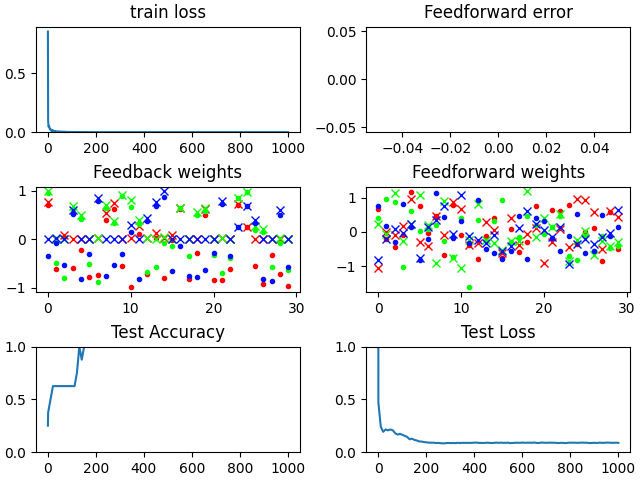
\includegraphics[width=0.8\textwidth]{fig_exc_inh_training}
    \caption{Training progress of a network of rate neurons in NEST, in which hidden layer connections between
        interneurons and pyramidal neurons are unipolar and nonspecific.}
    \label{fig-exc-inh-training}
\end{figure}


\section{In search of plausible spike frequencies}
\todo{expand}


\section{Resilience to imperfect connectivity}

\begin{figure}[t]
    \centering
    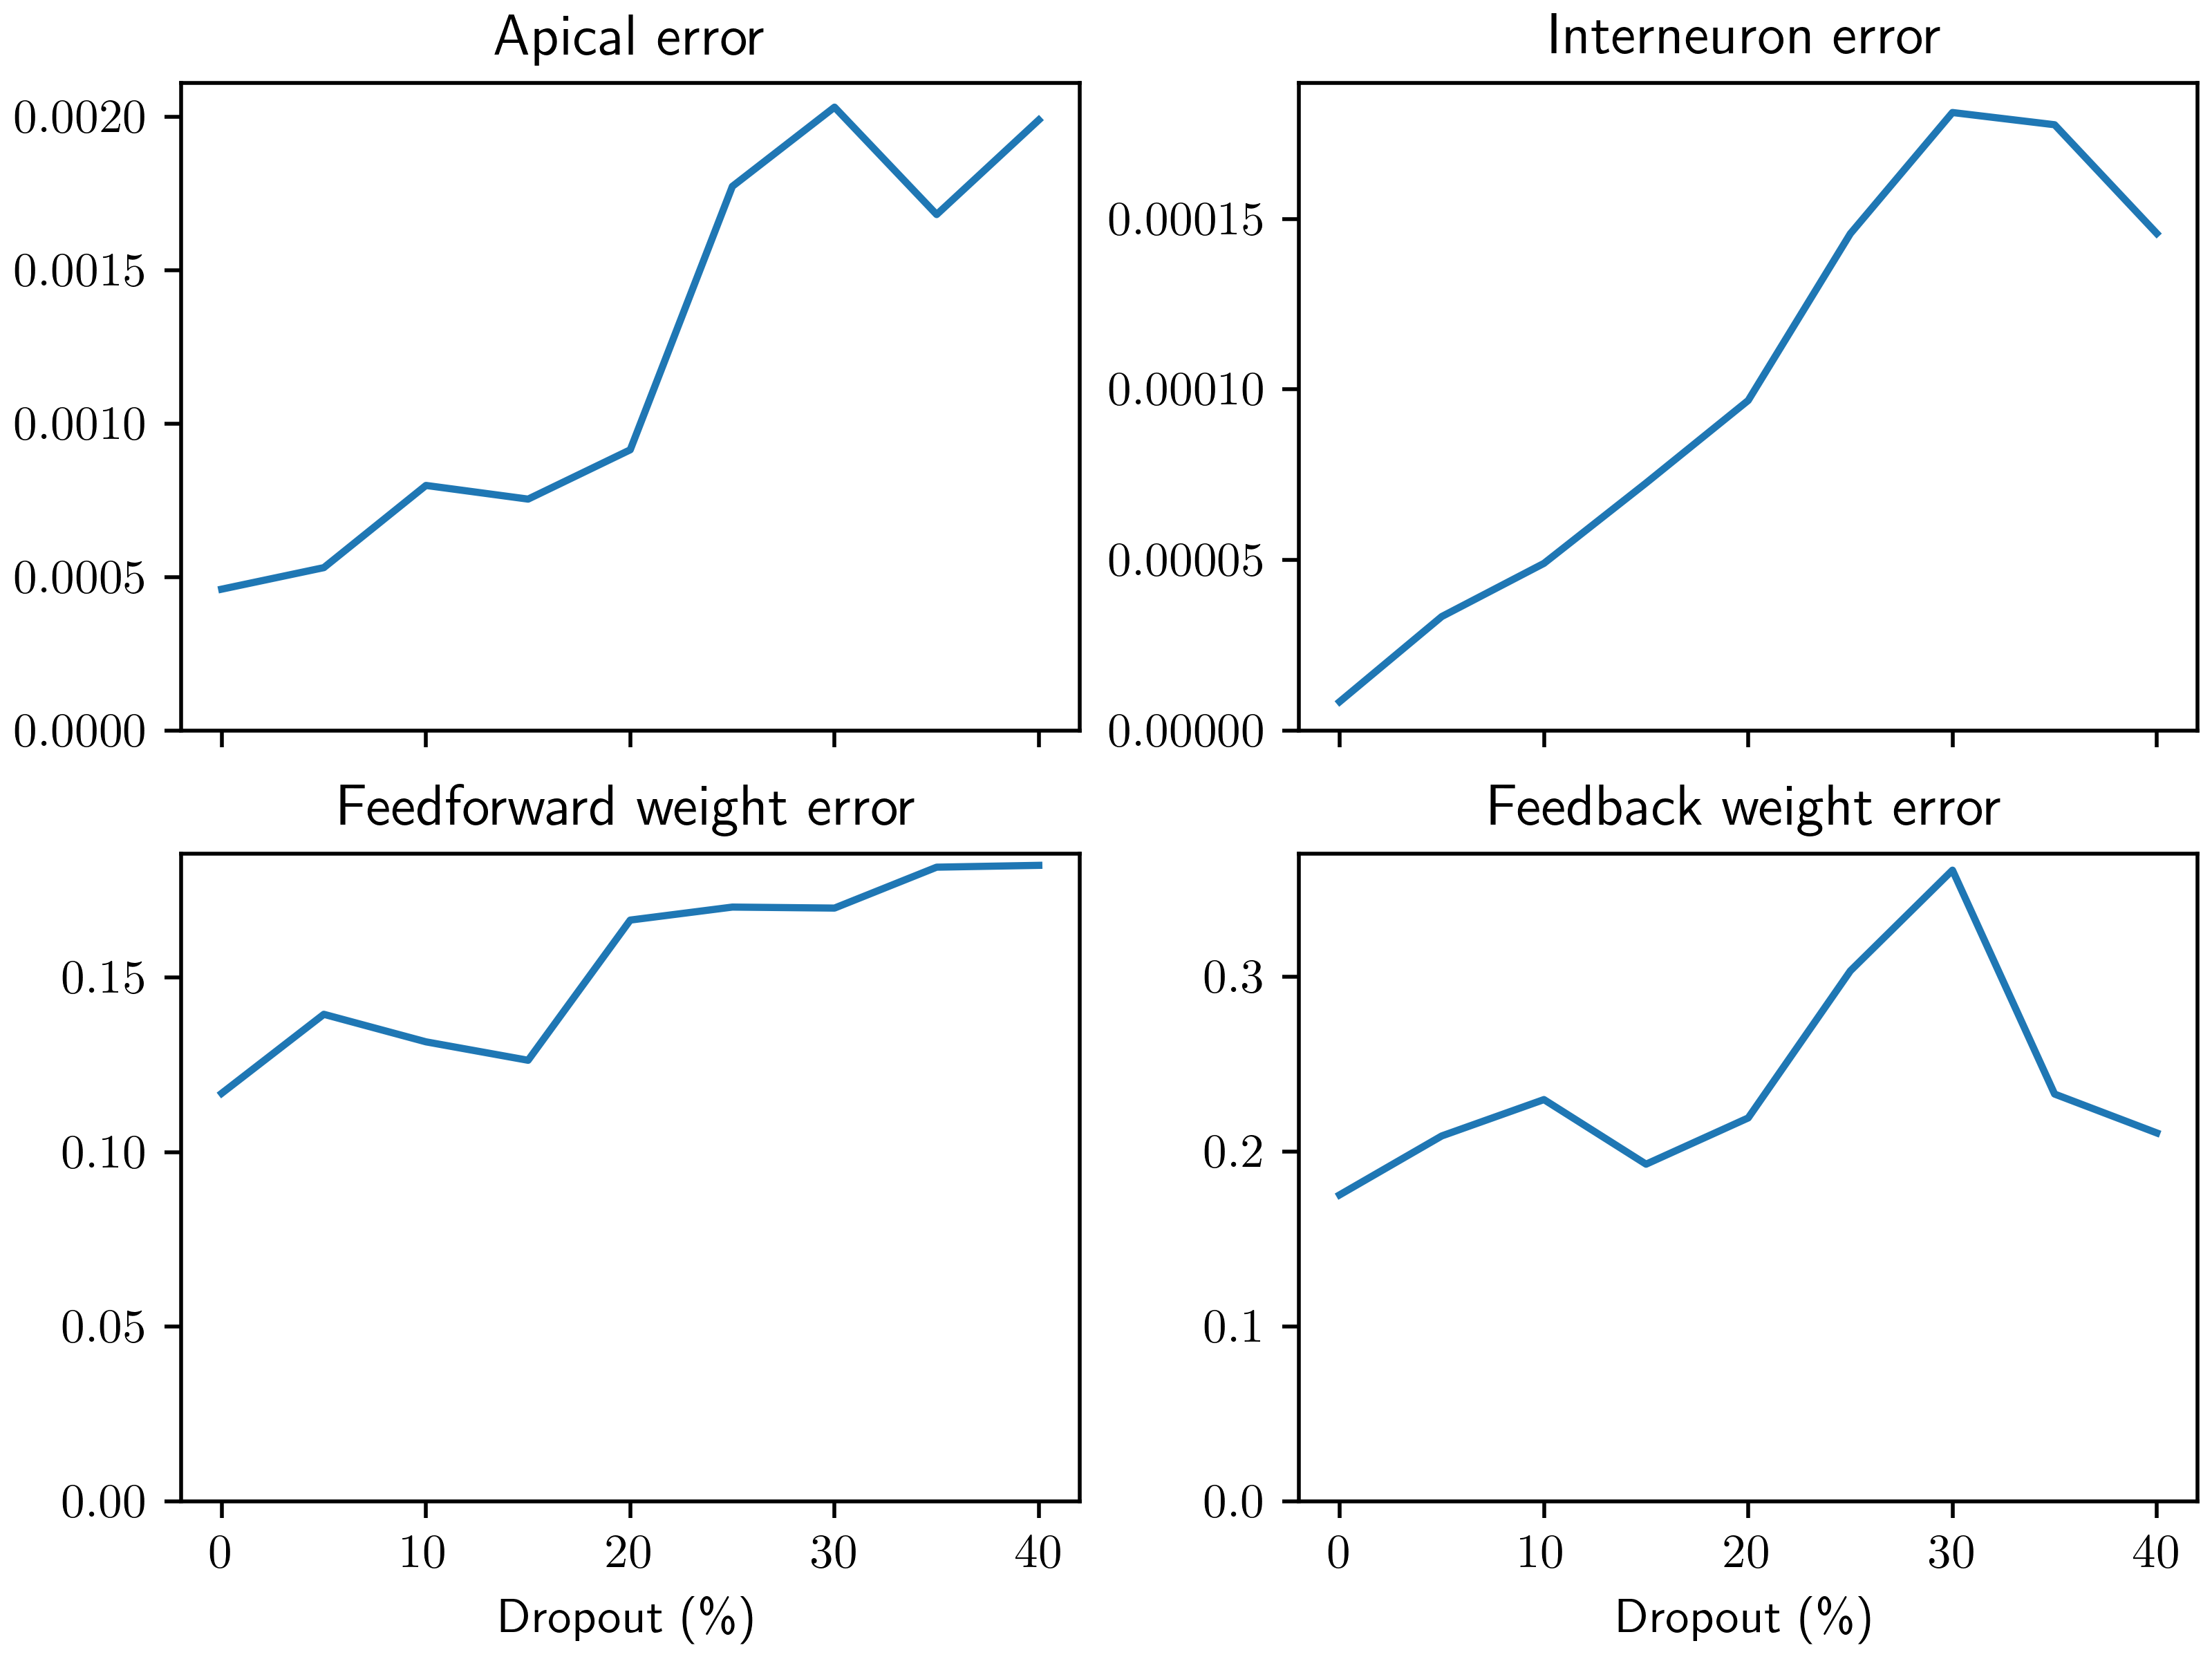
\includegraphics[width=0.9\textwidth]{fig_dropout}
    \caption{Error terms after training a network with dimensions [8, 8, 8] towards the self predicting states, with
        different percentages of synaptic connections randomly removed. To avoid completely separated layers, synapse
        deletion was performed per synaptic population, and the percentage is therefore only an approximation. Even with
        only 60\% of synaptic connections present, the network architecture still achieves competetive values for all four
        error metrics. For the weight errors, which is calculated with MSE over two matrices, missing
        synapses were set to $0$. This choice was made under the assumption that a missing connection in an ideal
        self-predicting network would be matched by a zero-weight - or likewise absent - synapse. Experiments were performed
        with the rate-based network in NEST, each network was trained fro 2000 epochs of 50ms each.}
    \label{fig-dropout}
\end{figure}


\section{direct feedback connections to interneurons}\label{sec-electric-syns}

\cite{Vaughn2022,Mancilla2007}



\section{Performance of the different implementations}\label{sec-benchmark}

As stated in \cite{Haider2021}, simulating the present network with many neurons or more than one hidden layer quickly
becomes unfeasible when simulating the full leaky dynamics. To investigate how network size affects simulation time, all
three implementations created for this project were trained on the bars dataset for a single epoch with different
network sizes for a single epoch, in order to assess efficiency.


\begin{figure}[t]
    \centering
    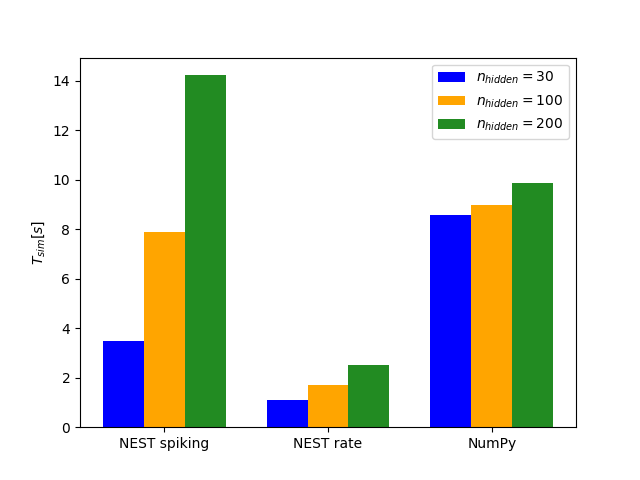
\includegraphics[width=0.8\textwidth]{fig_benchmark}
    \caption{Benchmark of the three different implementations using a network of $[9, n_{hidden}, 3]$ neurons per layer.
        $n_{hidden}=30$ was chosen as a baseline, as it is the default throughout all simulations on the Bars dataset.
        Networks were instantiated with the same synaptic weights and trained for a single epoch of 5 stimulus
        presentations of $100ms$ each. Simulations were performed on an \textit{AMD Ryzen Threadripper 2990WX} using 8
        cores for the NEST simulations at up to $3.0GHz$.}
    \label{fig-benchmark}
\end{figure}

The result of this comparison is shown in Fig. \ref{fig-benchmark}. The NumPy network is slow at baseline, which is
likely explained by the fact that it is the only variant which is running on a single thread. This is due to a
limitation of NumPy, and could likely be improved greatly by using batched matrix multiplications, as are provided for
example by \texttt{PyTorch}\footnote{It is also possible, that the network code surrounding the NumPy computations is
    less efficient than the one for the NEST network. As this implementation was needed primarily to prove that neuron
    dynamics and synaptic updates were ported correctly to NEST, efficiency was a minor concern here and this was not
    investigated further.}.  Notably, this variant exhibits very little slowdown in response to an increase in network size.
My assumption is, that the vectorization of synaptic updates on a single thread scales up better than the communication
between threads that is required by most events in the NEST simulations. The NEST implementation using rate neurons
performed best in terms of speed across the board. This result was slightly surprising, as the demand on the
communication interface between threads is very high, since all neurons transmit an event to each of their postsynaptic
targets at every time step.

Finally, the novel spiking variant of this model performed substantially worse than anticipated. Particularly in
comparison to the rate implementation, I initially expected substantial performance improvements. The Difference between
the two was even greater when simulating on an office-grade processor (Benchmark was also run on an \textit{Intel Core
    i5-9300H} at $2.40GHz$, results not shown). Three hints about the comparatively poor performance can be deduced: For
one, both the rate and the spiking neuron model employ almost identical neuron models, with minor changes to
parametrization and output generation. Thus, updates to the neuron state are unlikely to be responsible for the worse
performance. Secondly, the number of Events transmitted between neurons is much lower for the SNN compared to

the \textit{relative} performance decrease when increasing the number neurons by the same amout is much greater for the
spiking network. Thus, the most likely cause of slowdown are the updates at the synapses. This is supported by the fact,
that the number of synapses increases much faster for this kind of network than the number of neurons. For the given
network of $n_{x} = 9$ input neurons, $n_y = 3$ output neurons and $n_{h}$ neurons in the hidden layer $l$, the number
of total synapses in the network is given by

\begin{align}
    n_{synapses} & = |w_{l}^{up}| + |w_{l}^{pi}| + |w_{l}^{ip}| + |w_{l}^{down}| + |w_{y}^{up}| \\
                 & = n_h n_x + n_h n_y + n_y n_h  + n_h n_y + n_y  n_h                          \\
                 & = n_h (n_x + n_y^4)
\end{align}

with $|w|$ of a weight matrix $w$ in this case denoting the total number of elements in that matrix \what{Is there a
    more conventional notation?}. Thus, the number of synapses in a network grows much faster than the number of total
neurons when increasing the size of the hidden layer.

availis given by the stark increase in

\section{Response to unpredicted stimuli}

The activity of many cortical neurons increases when a brain is presented with unpredicted stimuly that regard these
neurons \todo{check out \cite{whittington2019theories} refs 50-54}. This property is prominently replicated by
predictive coding networks, since activation of error nodes is a function of local prediction errors. Prediction errors
in the present model on the other hand are encoded in both positive and negative potentials of apical dendrites. Hence,
the

\begin{figure}[t]
    \centering
    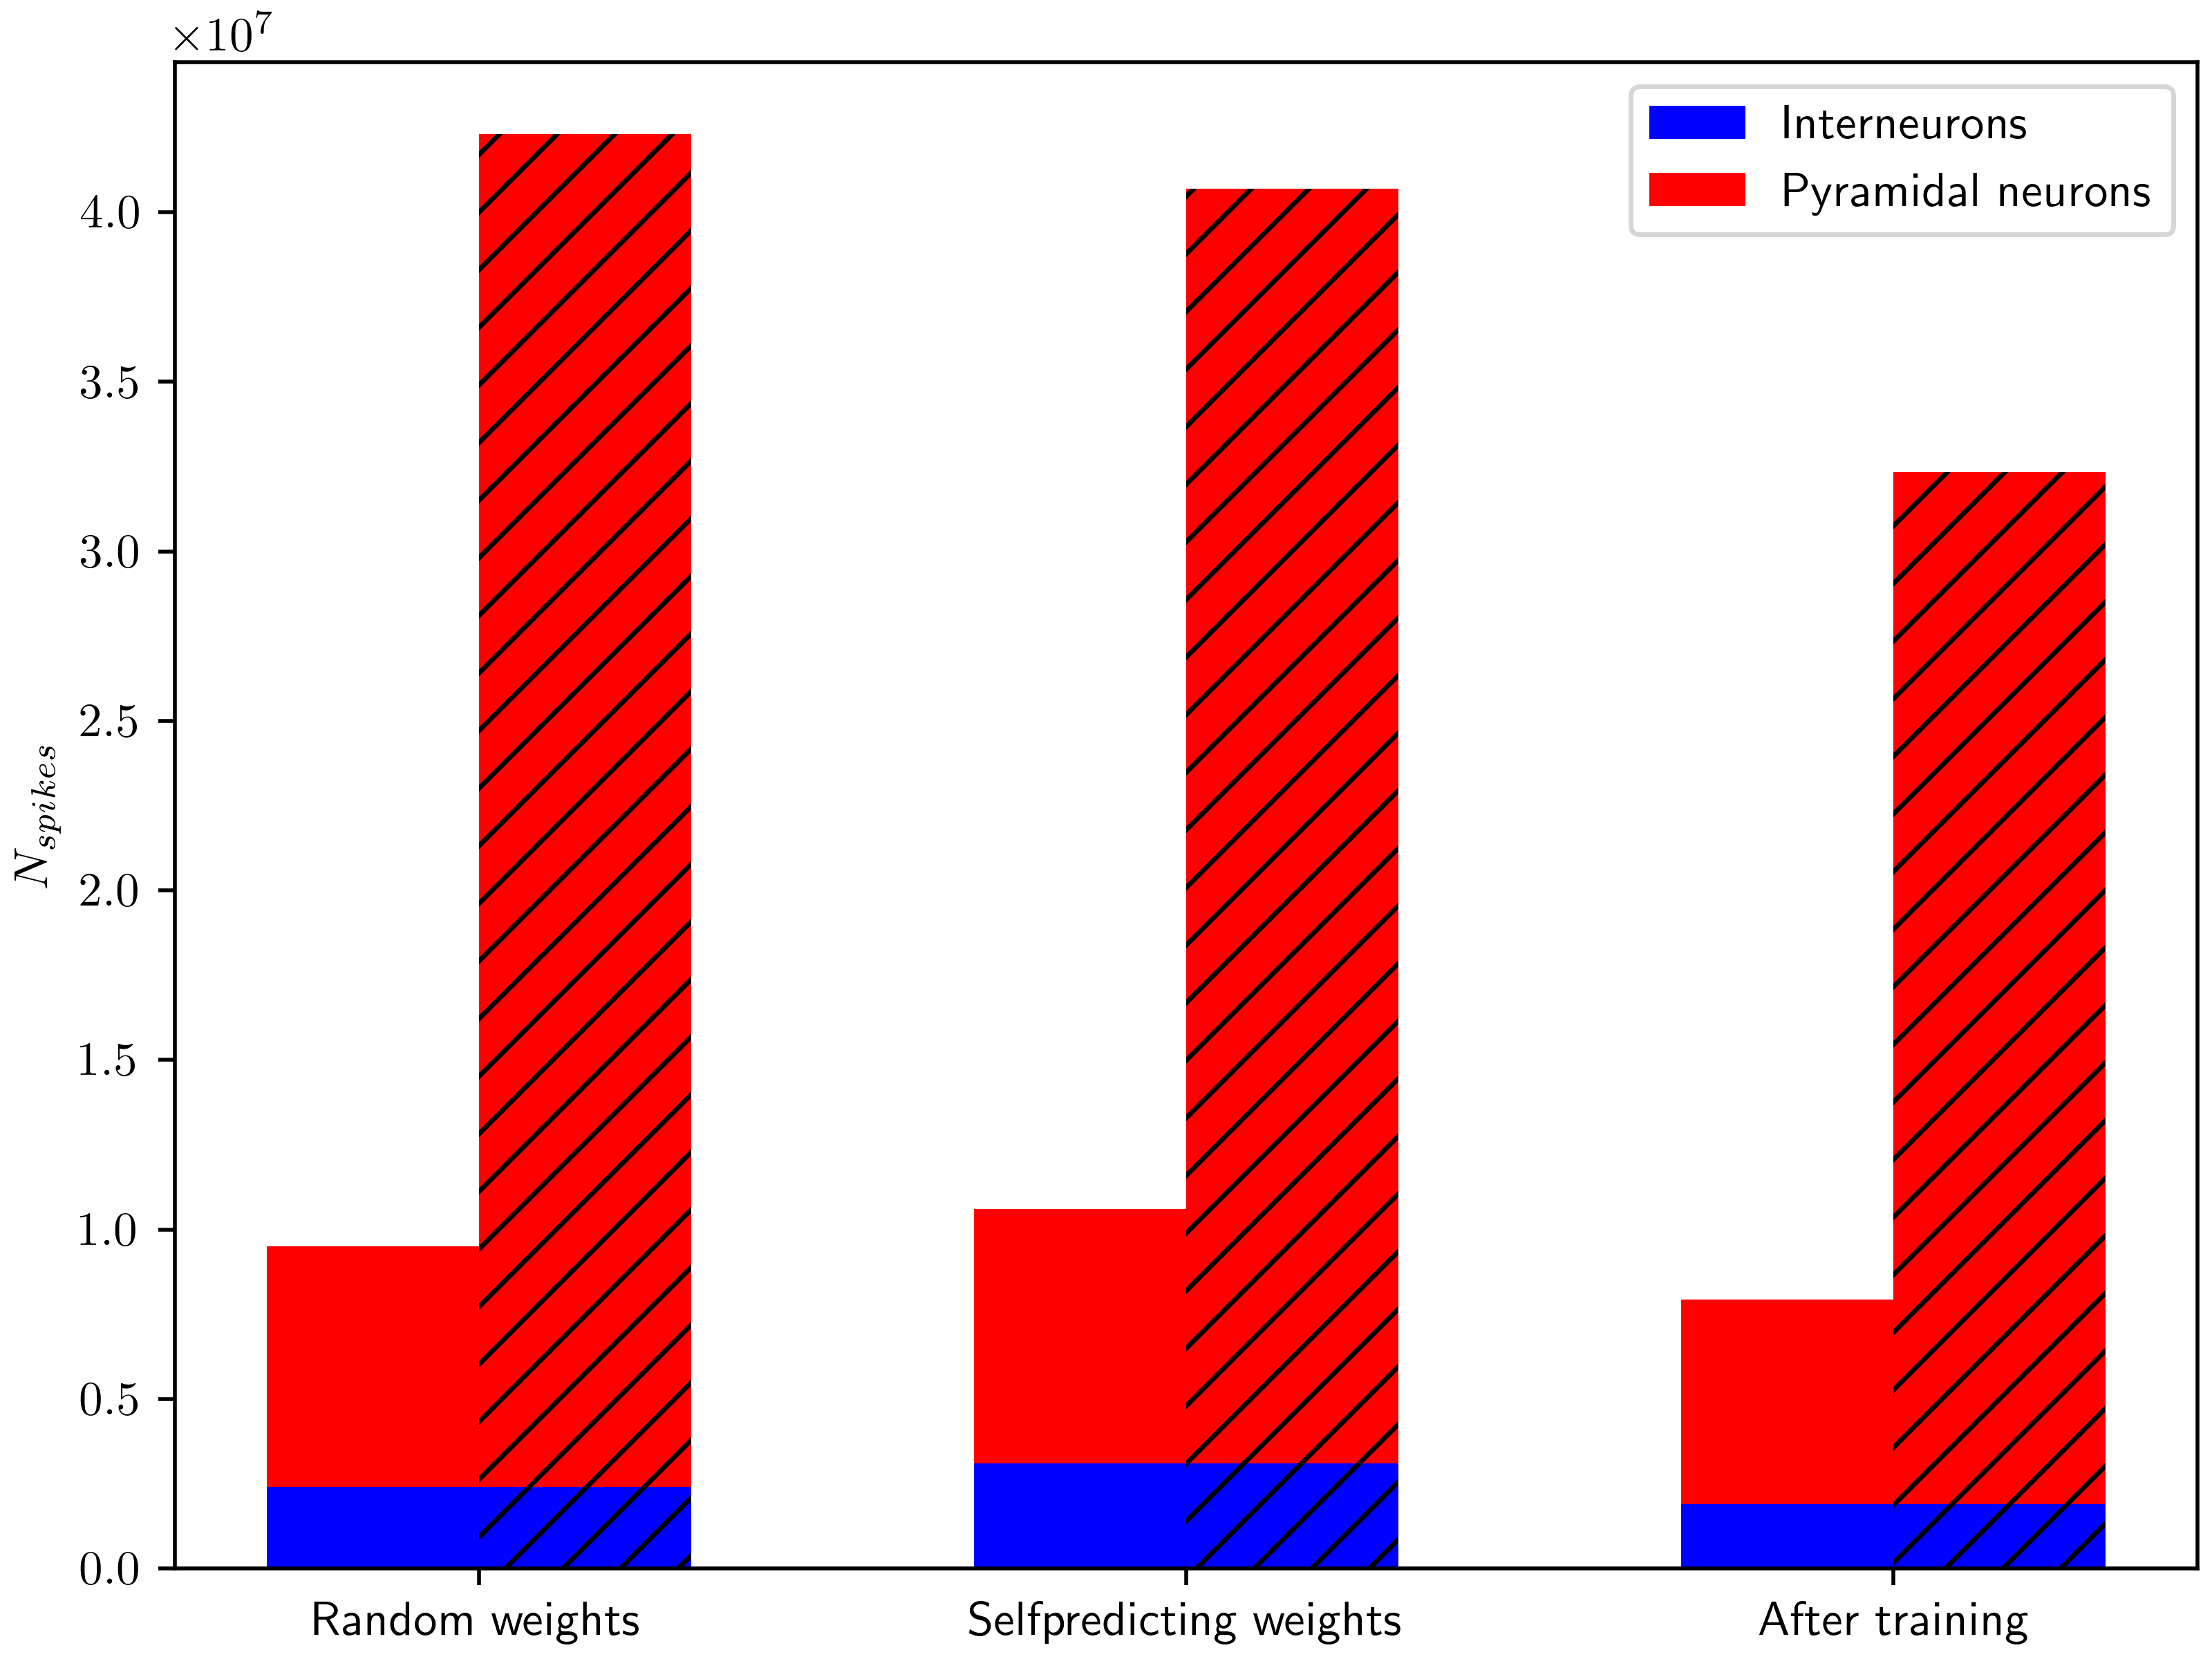
\includegraphics[width=0.9\textwidth]{fig_activity_unpredicted_stimulus}
    \caption{Comparison of network response to stimuli from the Bars dataset.}
    \label{fig-stimulus-response}
\end{figure}




